% mirko.rahn@itwm.fraunhofer.de

\documentclass[a4paper,12pt]{article}

\usepackage{tikz}\usetikzlibrary{automata,arrows,snakes,shapes,shadows}
\usepackage{amssymb}
\usepackage{amsmath}
\usepackage{ngerman}
\usepackage[latin1]{inputenc}
\usepackage[T1]{fontenc}
\usepackage{microtype}
\usepackage{fixltx2e}
\usepackage{tocloft}
\usepackage{ifthen}
\usepackage[nosepfour]{numprint}
\usepackage{url}
%\usepackage{zref-perpage}
\usepackage{index}
\usepackage{fancyhdr}
\usepackage{booktabs}
\usepackage{moreverb}
%\usepackage{citeref}
\usepackage{xspace}
\usepackage{mparhack}
%\usepackage[pdftex]{graphicx}
%\usepackage{thumbpdf,hyperref}

\parindent 0pt

\newlength{\lw}\setlength{\lw}{1pt}
\newlength{\st}\setlength{\st}{0pt}

\newcommand{\parens}[3]{#1#3#2}
\newcommand{\K}[1]{\parens{(}{)}{#1}}
\newcommand{\eps}{\varepsilon}

\tikzstyle{every picture}+=[>=angle 90]
\tikzstyle{every picture}+=[bend angle=10]
\tikzstyle{every picture}+=[auto]
\tikzstyle{every picture}+=[join=round]
\tikzstyle{every picture}+=[cap=butt]
\tikzstyle{every picture}+=[line width=\lw]
\tikzstyle{every picture}+=[double distance=2\lw]
\tikzstyle{every picture}+=[shorten >=\st]
\tikzstyle{every picture}+=[node distance=4em]
\tikzstyle{every loop}=[->,shorten >=\st]
\tikzstyle{tight}=[inner sep=0pt,outer sep=0pt]
\tikzstyle{zero}=[draw=none,coordinate]

\tikzstyle{trans}+=[draw, fill=white]
\tikzstyle{trans}+=[inner sep=0.5em,outer sep=0pt]
\tikzstyle{trans}+=[minimum height=2em]
\tikzstyle{trans}+=[drop shadow]

\tikzstyle{state}+=[fill=white]
\tikzstyle{state}+=[drop shadow]

\tikzstyle{every picture}+=[every shadow/.style={opacity=.8}]

\tikzstyle{invis}=[draw=none,inner sep=0pt,minimum height=0pt]

\newcommand{\type}[1]{\textsc{#1}}
\newcommand{\program}[1]{\textit{#1}}
\newcommand{\expression}[1]{\texttt{#1}}
\newcommand{\transition}[1]{\texttt{|#1|}}
\newcommand{\place}[1]{\texttt{(#1)}}
\newcommand{\port}[1]{\texttt{[#1]}}
\newcommand{\file}[1]{\textsl{file://#1}}
\newcommand{\element}[1]{\texttt{<#1>}}
\newcommand{\function}[1]{\texttt{<#1>}}
\newcommand{\attribute}[1]{\texttt{<#1>}}

\begin{document}

\title{Editor f"ur die Fraunhofer Parallel Programming Platform}

\author{Mirko Rahn\thanks{\texttt{mirko.rahn@itwm.fraunhofer.de},
    Telefon: +49(0)631/31600\,4553}}

\maketitle

\begin{abstract}
  Im Rahmen des MWARE MAVO produziert das ITWM eine neuartige
  Plattform zur schnellen grafischen Entwicklung f"ur und effizienten
  Ausf"uhrung paralleler Programme auf HPC Systemen.

  Wir stellen zun"achst in sehr knapper Form die Plattform vor, die
  von Workflows gesteuert wird, die als Petri-Netz formuliert
  werden. Wir gehen auf die Erweiterungen ein, die wir gegen"uber
  \glqq normalen\grqq\ Petri-Netzen eingebaut haben. Unser
  Austauschformat und bereits vorhandene Programme werden kurz
  beleuchtet.
  
  Zum Editor stellen wir ausgehend vom Stand der Dinge insgesamt drei
  Anwendungsszenarien vor, die sich jeweils immer weiter von den
  Details der Plattform entfernen.

  Neben dem Editor ist der Monitor ein wichtiger Baustein. Wir stellen
  kurz unsere Vorstellungen dar.
\end{abstract}

\clearpage
\tableofcontents
\clearpage

\section{Die Plattform}

Wesentliche Idee ist die Trennung von Koordinierungsprache und
Programmiersprache oder besser Berechnungssprache. Auf der Ebene der
Berechnungssprache sprechen wir "uber Module, die Daten konkret
bearbeiten, "uber Algorithmen. Diese Module wollen und sollen sich
aber nicht k"ummern um zum Beispiel das Herbeischaffen der
Eingabedaten, das Speichern oder Weiterleiten der Ausgabedaten. Das
sind Aufgaben, die auf der Ebene der Koordinierungssprache erledigt
werden. Ebenfalls zur Koordinierung geh"oren (automatische)
Parallelisierung, (automatische) Balancierung der Last, (automatische)
Fehlertoleranz, "Uberwachung des Systems, \ldots \cite{gelernter}

\begin{figure}
\begin{center}
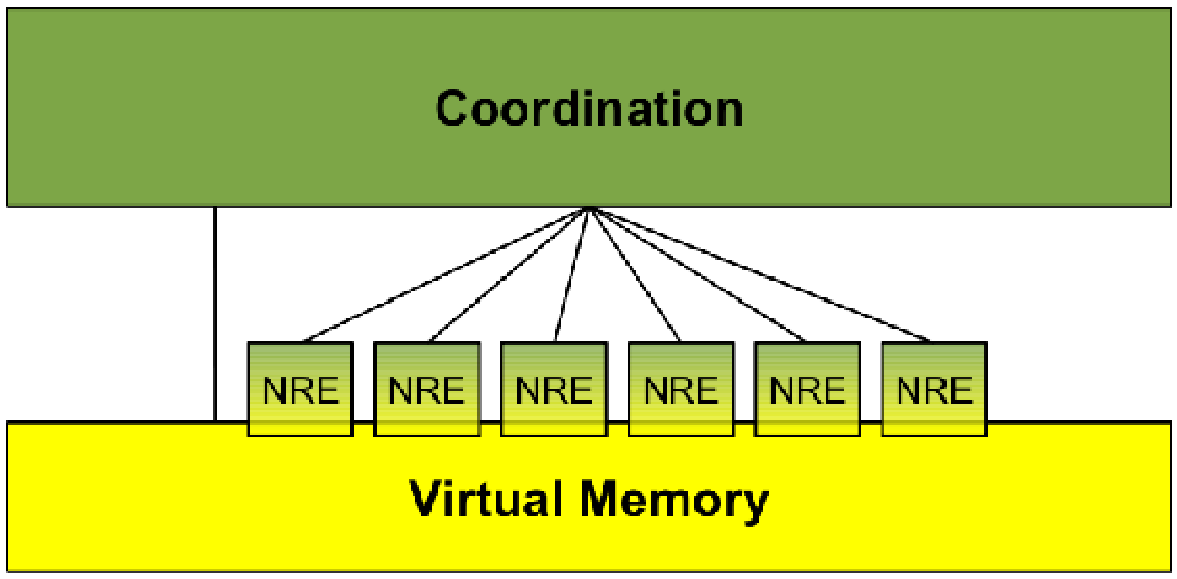
\includegraphics[width=0.8\textwidth]{architecture.pdf}
\end{center}
\caption{Architektur der Plattform}\label{fig:arch}
\end{figure}

In Abbildung \ref{fig:arch} ist die grundlegende Architektur der
Plattform dargestellt: Die Koordinierungsschicht kontrolliert eine
Reihe von Knoten (NRE = node runtime environment), die auf einem
virtuellen Speicher aufsitzen. Der virtuelle Speicher verwendet GPI
uns stellt einen partitionierten globalen Adressraum zur
Verf"ugung. Die Komponenten haben alle jeweils Substrukturen, die hier
aber nicht weiter betrachtet werden sollen.

Die Plattform trifft keine Annahmen "uber die Berechnungsebene. Ein
Modul muss lediglich als dynamisch linkbare Objektdatei vorliegen und
seine Parameterliste der Koordinierungsschicht bekannt machen.

Die Koordinierungsschicht wird von Workflows gesteuert. Ein Workflow
ist ein Petri-Netz, genauer ein getyptes (gef"arbtes) hierarchisches
Petri-Netz.

\section{Petri-Netze}

Petri-Netze sind wohlbekannt und werden in der Informatik, im
Schaltungsdesign und auch als Proze\3beschreibungssprache erfolgreich
eingesetzt. Sie haben viele Vorteile, insbesondere sind sowohl
Kontroll- als auch Datenflu\3 explizit dargestellt und Parallelit"at
ist direkt und nat"urlich im Netz abgebildet. Dar"uber hinaus sind
Petri-Netze gut erforscht und es gibt jede Menge Theorie, die f"ur
gute Praxis ja unerl"a\3lich ist. Schlie\3lich kann der Zustand eines
laufendes Workflows auf nat"urliche Weise im definierenden Petri-Netz
dargestellt werden.

\subsection{Pl"atze, Token und Transitionen}

Ein Petri-Netz besteht aus Pl"atzen und Transitionen. Transitionen
repr"asentieren Module bzw.\ Algorithmen. Transitionen sind durch
gerichtete Kanten sind Pl"atzen verbunden. Auf Pl"atzen k"onnen Token
liegen. Token repr"asentieren Daten.

Liegen auf allen Eingangspl"atzen einer Transition Token, dann kann
diese Transition schalten. Beim Schalten konsumiert die Transition
einen Token von jedem Eingangsplatz und produziert einen Token auf
jedem Ausgangsplatz. Wenn gleichzeitig mehrere Transitionen schalten
k"onnen, wird eine zuf"allig ausgew"ahlt.

Wir werden nun ausgehend von einfachen Netzen, die einzelnen
Erweiterungen darstellen, die die Plattform vornimmt.

\subsection{Einfache Netze}

\begin{center}
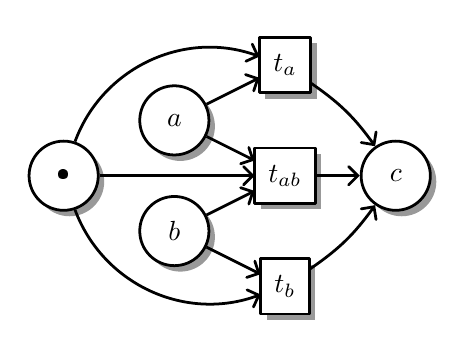
\begin{tikzpicture}
\node[invis] (z) {};
\node[state] (trigger) [left of=z, node distance=4em] {\textbullet};
\node[state] (a) [above of=z, node distance=2em] {$a$};
\node[state] (b) [below of=z, node distance=2em] {$b$};

\node[trans] (t_ab) [right of=z] {$t_{ab}$};
\node[trans] (t_a) [above of=t_ab] {$t_{a}$};
\node[trans] (t_b) [below of=t_ab] {$t_{b}$};

\node[state] (c) [right of=t_ab] {$c$};

\path[->]
   (a) edge (t_a)
   (a) edge (t_ab)
   (b) edge (t_b)
   (b) edge (t_ab)
   (t_a) edge [bend left] (c)
   (t_b) edge [bend right] (c)
   (t_ab) edge (c)
;
\path[->, bend angle=45]
   (trigger) edge (t_ab)
   (trigger) edge [bend left] (t_a)
   (trigger) edge [bend right] (t_b)
;
\end{tikzpicture}
\end{center}

Man "uberlege sich, dass dieses Netz genau dann einen Token auf dem
Platz $c$ produziert, wenn auf den Pl"atzen $a$ oder $b$ Token liegen.

\subsection{Ausdr"ucke}

Wir haben in der Workflow-Engine einen Expression-Parser und
-Evaluator eingebaut. Es handelt sich um eine einfache Sprache mit
logischen (und, oder, nicht), komparativen ($<$, $\le$, $>$, $\ge$,
$\ne$, $=$) und arithmetischen ($+$, $-$, $\times$, $/$, $\%$, \^{},
$\min$, $\max$, $\mbox{abs}$, $\mbox{floor}$, $\mbox{ceil}$,
$\mbox{round}$, $\mbox{sin}$, $\mbox{cos}$, $\mbox{sqrt}$, $\log$)
Operationen. Es gibt die M"oglichkeit zu verzweigen
(if-then-else). Die genaue Spezifikation dieser (noch etwas
m"achtigeren) Sprache soll jetzt nicht dargestellt werden, sie
funktioniert aber nach dem Prinzip der kleinsten "Uberraschung.

Ausdr"ucke k"onnen direkt in einer Transition angegeben werden um
kleinere Rechungen durchzuf"uhren.

\begin{center}
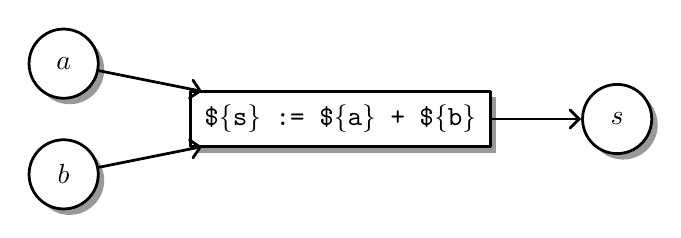
\begin{tikzpicture}
\node[invis] (z) {};
\node[state] (a) [above of=z, node distance=2em] {$a$};
\node[state] (b) [below of=z, node distance=2em] {$b$};

\node[trans] (sum) [right of=z, node distance=10em] {\expression{\$\{s\} := \$\{a\} + \$\{b\}}};

\node[state] (s) [right of=sum, node distance=10em] {$s$};

\path[->]
   (a) edge (sum)
   (b) edge (sum)
   (sum) edge (s)
;
\end{tikzpicture}
\end{center}

\subsection{Bedingungen}\label{sec:cond}

Transitionen k"onnen Vorbedingungen formulieren, die erf"ullt sein
m"ussen, damit die Transition schaltet. Die Bedingungen werden in der
selben Sprache formuliert wie die Ausdr"ucke.

\begin{center}
\begin{tikzpicture}
\node[invis] (z) {};
\node[state] (i) [above of=z, node distance=2em] {$i$};
\node[state] (m) [below of=z, node distance=2em] {$m$};

\node[trans] (init) [left of=z, node distance=8em] {$\begin{array}{l}\mbox{\expression{\$\{i\} := 0;}}\\\mbox{\expression{\$\{m\} := \$\{N\}}}\end{array}$};
\node[trans] (step) [right of=z, node distance=10em] {$\begin{array}{l}\mbox{Bedingung: \expression{\$\{i\} < \$\{m\}}}\\\mbox{\expression{\$\{x\} := \$\{i\};}}\\\mbox{\expression{\$\{i\} := \$\{i\} + 1}}\end{array}$};
\node[trans] (break) [below left of=step, node distance=8em] {Bedingung: \expression{\$\{i\} >= \$\{m\}}};

\node[state] (N) [above of=init, node distance=6em] {$N$};
\node[state] (x) [above of=sum, node distance=6em] {$x$};

\path[->, bend angle=5]
   (i) edge [bend left] (step)
   (m) edge [dashed] (step)
   (step) edge [bend left] (i)
   (step) edge (x)
   (i) edge (break)
   (m) edge (break)
   (init) edge (i)
   (init) edge (m)
   (N) edge (init)
;
\end{tikzpicture}
\end{center}

Wird auf den Platz $N$ eine Zahl $n$ gelegt, dann erzeugt dieses Netz
auf dem Platz $x$ die Zahlen von 0 bis $n-1$ in dieser Reihenfolge.

Eine weitere Erweiterung ist hier zu sehen: Die gestrichelte Kante vom
Platz $m$ ist eine Lesekante. Schaltet die rechte obere Transition,
dann wird der Token vom Platz $m$ \emph{nicht} entfernt. Er verbleibt
auf dem Platz $m$. Erst die untere Transition entfernt den Token vom
Platz $m$.

\subsection{Ports}

Bei den bisherigen Beispielen von Ausdr"ucken und Bedingungen war es
notwendig, innerhalb der Transition die Namen der angeschlossenen
Pl"atze zu kennen. Soll nun eine eigentlich gleiche Transition an
mehreren Stellen in einem Netz verwendet werden, m"ussten bei jeder
Verwendung an den Ausdr"ucken und den Bedingungen "Anderungen
vorgenommen werden. Dieses Problem l"osen wir mit dem Konzept des
Ports.

Ein Port ist dabei Ein- oder Ausgang in eine Transition, der einen
Namen hat. Innerhalb der Transition arbeiten Ausdr"ucke und
Bedingungen nur mit diesen Namen. Die Worflow-Engine "ubersetzt die
Namen der von au\3en angeschlossenen Pl"atze in die internen Namen.

Die Transition \emph{dup}

\begin{center}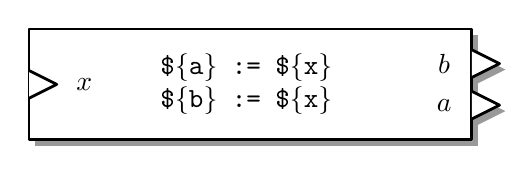
\begin{tikzpicture}
\draw[fill=white,drop shadow] (-8em,-2em) rectangle (8em,2em);

\draw (0pt,0pt) node {{\tt \begin{tabular}{l}\$\{a\} := \$\{x\}\;\\\$\{b\} := \$\{x\}\;\end{tabular}}};

\draw[fill=white] (-8em,0.5em) -- (-7em,0em) -- (-8em,-0.5em);
\draw (-6em,0em) node {$x$};

\draw[fill=white,drop shadow] (8em,1.25em) -- (9em,0.75em) -- (8em,0.25em);
\draw[fill=white,drop shadow] (8em,-0.25em) -- (9em,-0.75em) -- (8em,-1.25em);
\draw (7em,-0.75em) node {$a$};
\draw (7em,0.75em) node {$b$};
\end{tikzpicture}\end{center}

mit dem Eingangsport $x$ und den Ausgangsports $a$ und $b$ kann nun
zum Beispiel so mehrfach verwendet werden:

\begin{center}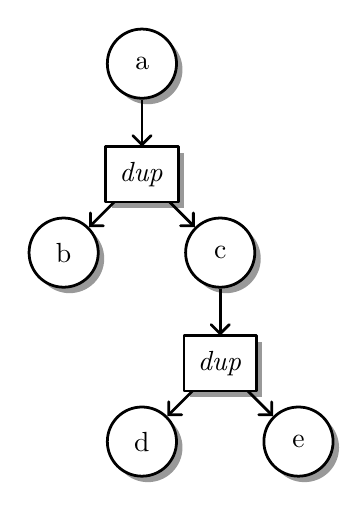
\begin{tikzpicture}
\node[state] (x) {a};
\node[trans] (dup1) [below of=x] {\emph{dup}};
\node[state] (x1) [below left of=dup1] {b};
\node[state] (x2) [below right of=dup1] {c};
\node[trans] (dup2) [below of=x2] {\emph{dup}};
\node[state] (x3) [below left of=dup2] {d};
\node[state] (x4) [below right of=dup2] {e};

\path[->]
  (x) edge (dup1)
  (dup1) edge (x1)
  (dup1) edge (x2)
  (x2) edge (dup2)
  (dup2) edge (x3)
  (dup2) edge (x4)
  ;
\end{tikzpicture}\end{center}

Beachte, dass beide Inkarnation von \emph{dup} intern die selben
Ausdr"ucke verwenden aber die Namen der angeschlossenen Pl"atze
verschieden sind.

\subsection{Typen}

Neben der Wiederverwendbarkeit ist die Typsicherheit ein wichtiger
Aspekt. Was zum Beispiel w"urde passieren, wenn auf den Platz $N$ im
Netz aus dem Abschnitt \ref{sec:cond} keine Zahl, sondern zum Beispiel
ein String gelegt wird? Was w"urde dann die Bedingung \expression{\$\{i\}
  < \$\{m\}} bedeuten?

Solche Situationen werden zuverl"assig verhindert, weil alle Pl"atze,
alle Token und alle Ports einen Typ haben.

Ein Platz vom Typ $T$ kann nur Token des selben Typs $T$
enthalten. Versucht eine Transition einen Token anderen Typs zu
platzieren wird der Workflow mit einer Ausnahme beendet.

Ein Platz von Typ $T$ kann nur mit einem Port vom Typ $T$ verbunden
werden.

Alle Ausdr"ucke und Bedingungen beachten die Typen der beteiligten
Operanden. Es zum Beispiel ist nicht m"oglich, Zahlen mit Strings zu
vergleichen.

Die Transition \emph{sum}

\begin{center}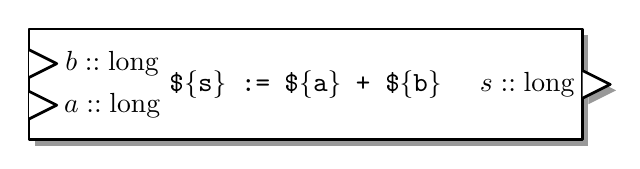
\begin{tikzpicture}
\draw[fill=white,drop shadow] (-10em,-2em) rectangle (10em,2em);

\draw (0pt,0pt) node {{\tt \$\{s\} := \$\{a\} + \$\{b\}}};

\draw[fill=white] (-10em,1.25em) -- (-9em,0.75em) -- (-10em,0.25em);
\draw[fill=white] (-10em,-0.25em) -- (-9em,-0.75em) -- (-10em,-1.25em);
\draw (-7em,-0.75em) node {$a::\mbox{long}$};
\draw (-7em,0.75em) node {$b::\mbox{long}$};

\draw[fill=white,drop shadow] (10em,0.5em) -- (11em,0em) -- (10em,-0.5em);
\draw (8em,0em) node {$s::\mbox{long}$};
\end{tikzpicture}\end{center}

kann zwei Zahlen des Typs \type{long} addieren und produziert eine
Zahl des Typs \type{long}. Dieser Workflow

\begin{center}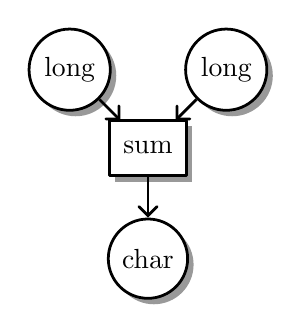
\begin{tikzpicture}
\node[state] (a) {long};
\node[trans] (sum) [below right of=a] {sum};
\node[state] (b) [above right of=sum] {long};
\node[state] (s) [below of=sum] {char};

\path[->]
  (a) edge (sum)
  (b) edge (sum)
  (sum) edge (s)
  ;
\end{tikzpicture}\end{center}

ist illegal kommt nicht zur Ausf"uhrung.

Die Workflow-Engine hat eine Reihe von Typen vordefiniert
(\type{control}, \type{bool}, \type{long}, \type{double},
\type{char}, \type{std::string}, \type{bitsetofint::type}) und
erlaubt die Definition eigener strukturierter rekursiver
Datentypen. Auch selbst definierte Typen unterliegen der strikten
Typpr"ufung.

\subsection{Externe Module}

Bisher haben wir nur "uber Transitionen gesprochen, die Ausdr"ucke
enthalten und innerhalb der Workflow-Engine bearbeitet werden. Die
eigentliche Arbeit wird von externen Modulen erledigt, die als
dynamisch linkbarer Objektcode vorliegen. Im Petrinetz stellen wir
solche externen Module durch eine Transition (mit getypten Ports) dar,
die den Namen des Moduls und der aufzurufenden Funktion enth"alt.

\subsection{Hierarchische Netze}\label{sec:hierarchy}

Ein dritter und letzter Transitionstyp ist der des Subnetzes. Eine
Transition, die ein Subnetz enth"alt ist zun"achst eine ganz normale
Transition mit getypten Ports. Die Ports sind mit Pl"atzen des
enthaltenen Netzes assoziert. Kann die Transition schalten, dann
werden die Token von den Eingabepl"atzen auf die mit den
entsprechenden Ports assozierten Pl"atze des enthaltenen Netzes
kopiert. Das enthaltene Netz wird dann ausgef"uhrt und anschlie\3end
werden die Token von den mit Ausgangsports assozierten Pl"atzen des
enthaltenen Netzes auf die mit diesen Ports verbundenen Pl"atze
kopiert.

Ein Beispiel: Achtung! Dieses Bild wurde mit Hilfe von
\program{pnet2dot} aus Abschnitt \ref{sec:pnet2dot} und \program{dot}
automatisch erzeugt. Es ist sehr gro\3! Das Bild kann am Bildschirm
mit entsprechender Vergr"o\3erung aber problemlos (teilweise)
angesehen werden.

\begin{center}
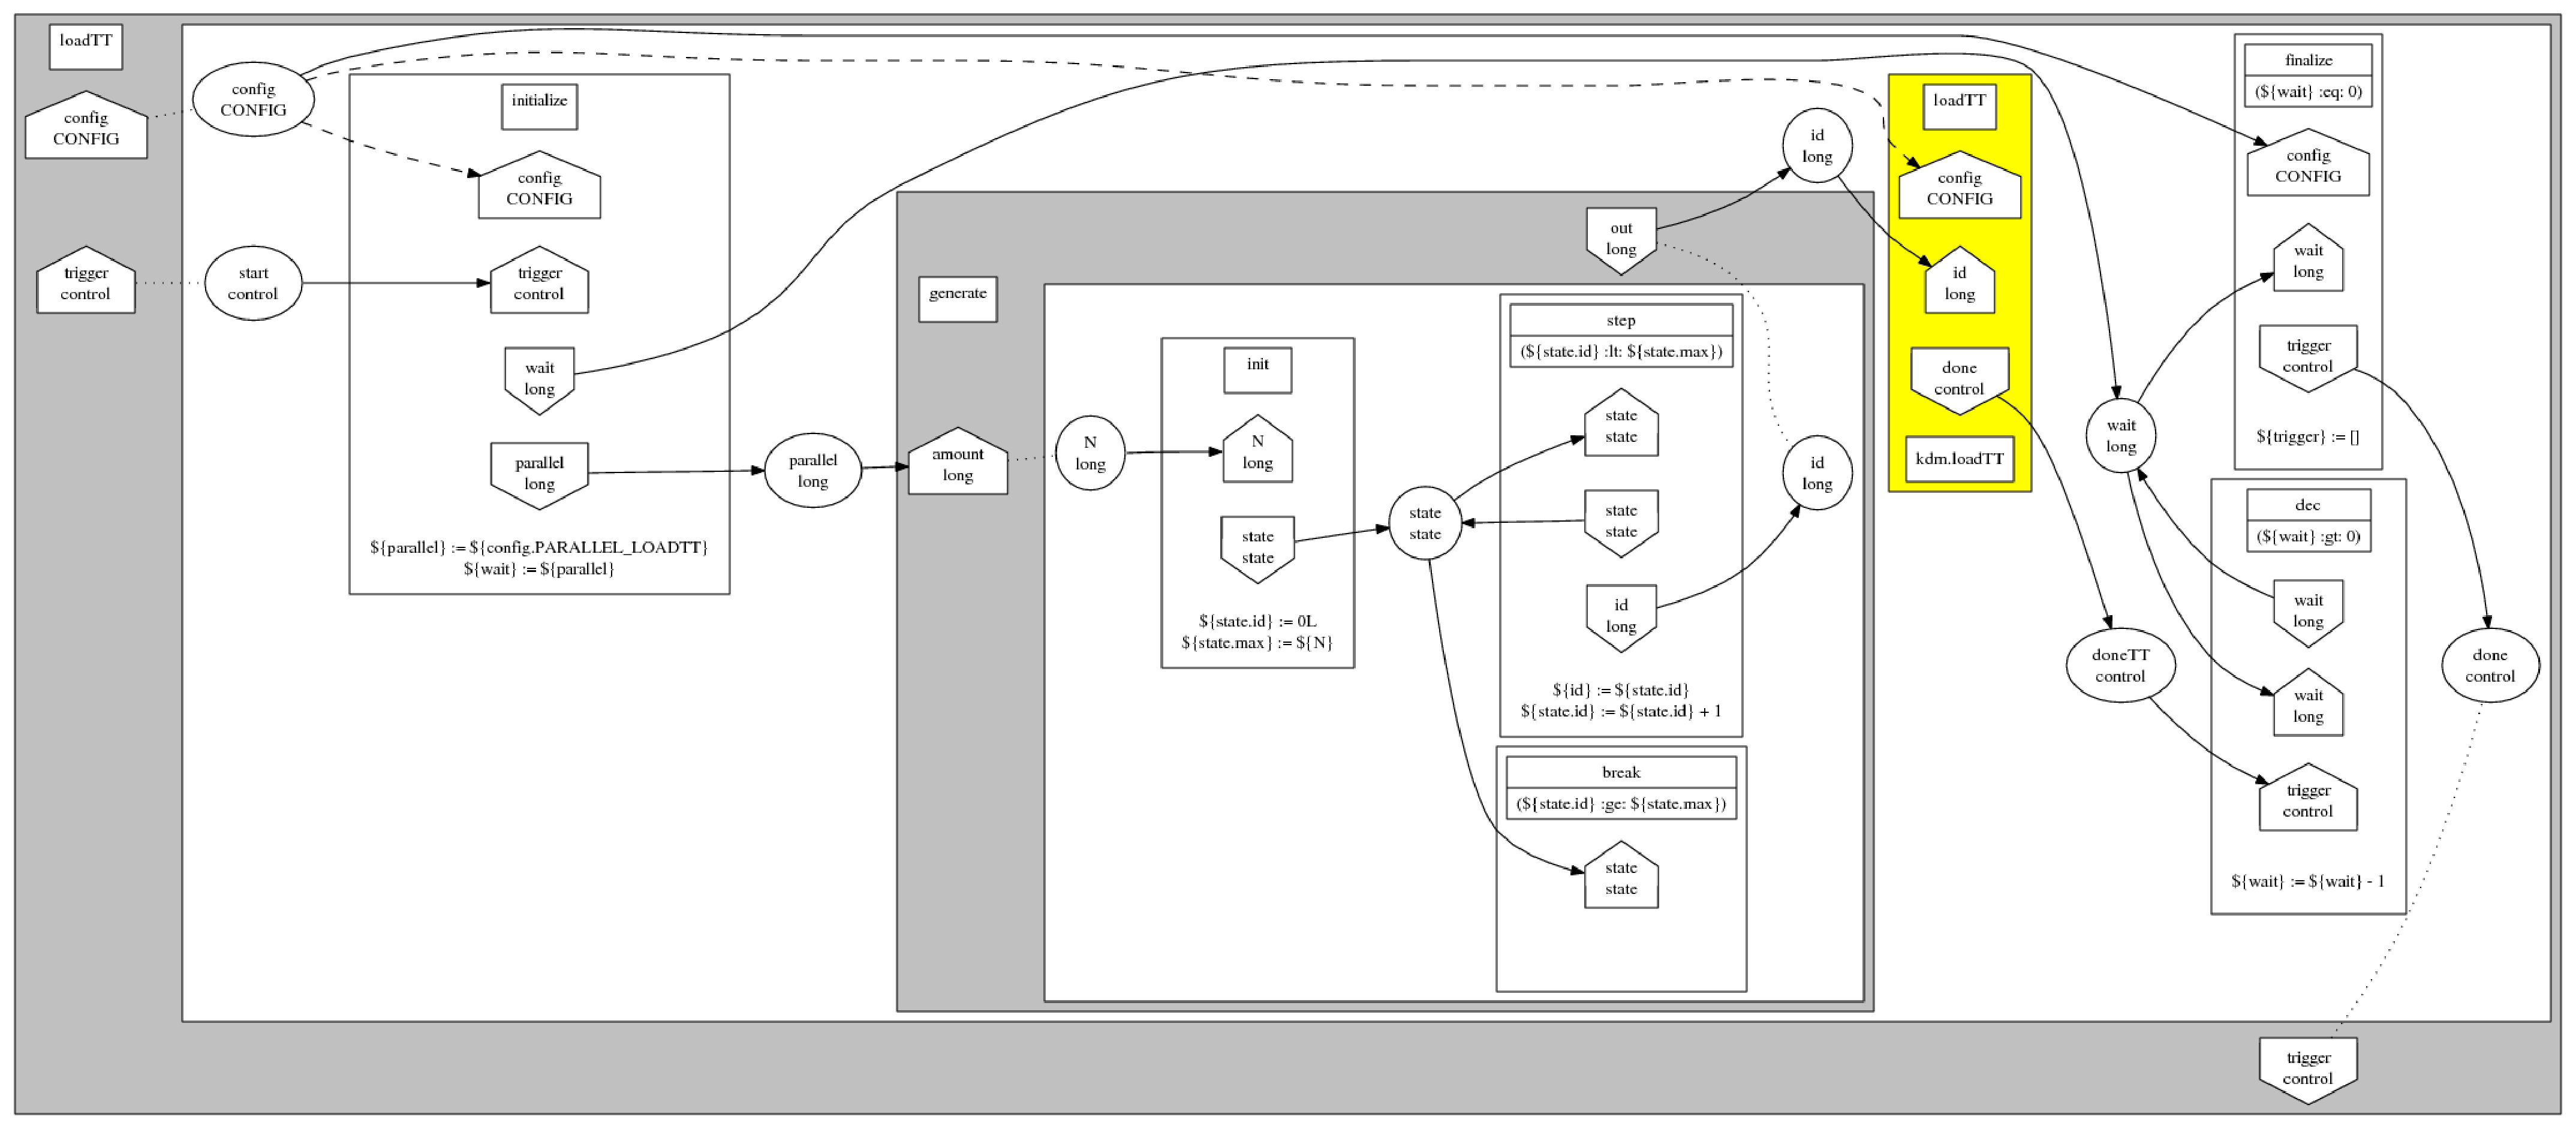
\includegraphics[width=\textwidth]{loadTT.pdf}
\end{center}

Die Notation hier ist die folgende: Pl"atze sind rund und haben einen
Namen und einen Typ. Transitionen sind rechteckig und haben einen
Namen und eventuell eine Bedingung, die beide in einem eingebetteten
Rechteck dargestellt sind. Innerhalb von Transitionen sind H"auser mit
Dach nach oben die Eingangsports und mit Dach nach unten die
Ausgangsports. Transitionen, die externe Module ansprechen sind gelb
hinterlegt und vermerken den Modulnamen und die aufzurufende
Funktion. Im Bild oben nur die gelbe Transition
\transition{loadTT}. Transitionen mit Ausdr"ucken geben den Ausdruck
einfach an. Im Bild oben hat die Transition \transition{dec} den
Eingangsport \port{trigger} mit dem Typ \type{control} und den
Eingangsport \port{wait} mit dem Typ \type{long}. Unter der
Bedingung, dass \expression{\$\{wait\} > 0} gilt, konsumiert die
Transition \transition{dec} je einen Token von den Pl"atzen \place{wait}
und \place{doneTT} und produziert auf dem Platz \place{wait} einen
neuen Token, der den Wert des alten verringert um eins enth\"alt.

Soweit zur Notation, nun zur hierarchischen Konstruktion. Die
Transition \transition{generate} hat den Eingangsport \port{amount} vom
Typ \type{long}, den Ausgangsport \port{out} ebenfalls vom Typ
\type{long} und enth"alt ein Subnetz. Der Eingansport \port{amount}
ist mit dem Platz \place{N} des Subnetzes assoziiert und der
Ausgangsport \port{out} mit dem Platz \place{id}.

Liegt nun auf dem Platz \place{parallel} ein Token (des Typs
\type{long}), dann kann die Transition \transition{generate}
schalten. Dieser Token wird dann auf den Platz \place{N} des
enthaltenen Netzes kopiert. Das innere Netz wird ausgef"uhrt, das
hei\3t, es darf arbeiten, bis keine Transition mehr schalten
kann. Anschlie\3end werden die Token vom Platz \place{id} des inneren
Netzes auf den Platz \place{id} des "au\3eren Netzes kopiert.

Im Bild oben ist die Transition \transition{generate} selbst Teil eines
Subnetzes innerhalb der grauen Transition \transition{loadTT}.

\subsubsection{Flachklopfen}

Hierarchische Netze sind ein sehr gutes konzeptionelles Mittel bei der
Konstruktion komplexer Netze, es gibt aber auch Probleme damit: Im
Beispiel aus Abschnitt \ref{sec:hierarchy} erzeugt die Transition
\transition{generate} die $n$ Token $0$, \ldots, $n-1$, wenn die Eingabe
der Wert $n$ ist. Erst nachdem alle diese Token erzeugt wurden, ist
die Arbeit des enthaltenen Netzes beendet und nun werden alle Token in
das "au\3ere Netz kopiert und sind erst dann im "au\3eren Netz
sichtbar. Ein Subnetz wird also nicht lazy ausgef"uhrt. Das Problem
ist offensichtlich: Was, wenn $n$ sehr gro\3 wird? Dann kopieren wir
sehr gro\3e Mengen von Token.

Im "ubrigen verh"alt sich die Transition \transition{generate} auch nicht
konform, denn eine Transition soll auf jedem Ausgabeplatz \emph{einen}
Token produzieren und nicht viele. Mit solchen Transitionen ist zum
Beispiel die Frage, ob ein Netz beschr"ankt ist, nicht mehr zu
beantworten.

Beide Probleme k"onnen wir durch Flachklopfen der Hierarchie
beheben. Diese Operation kann von unserem Compiler \program{pnetc} aus
Abschnitt \ref{sec:pnetc} durchgef"uhrt werden. Das Netz sieht dann so
aus:

\begin{center}
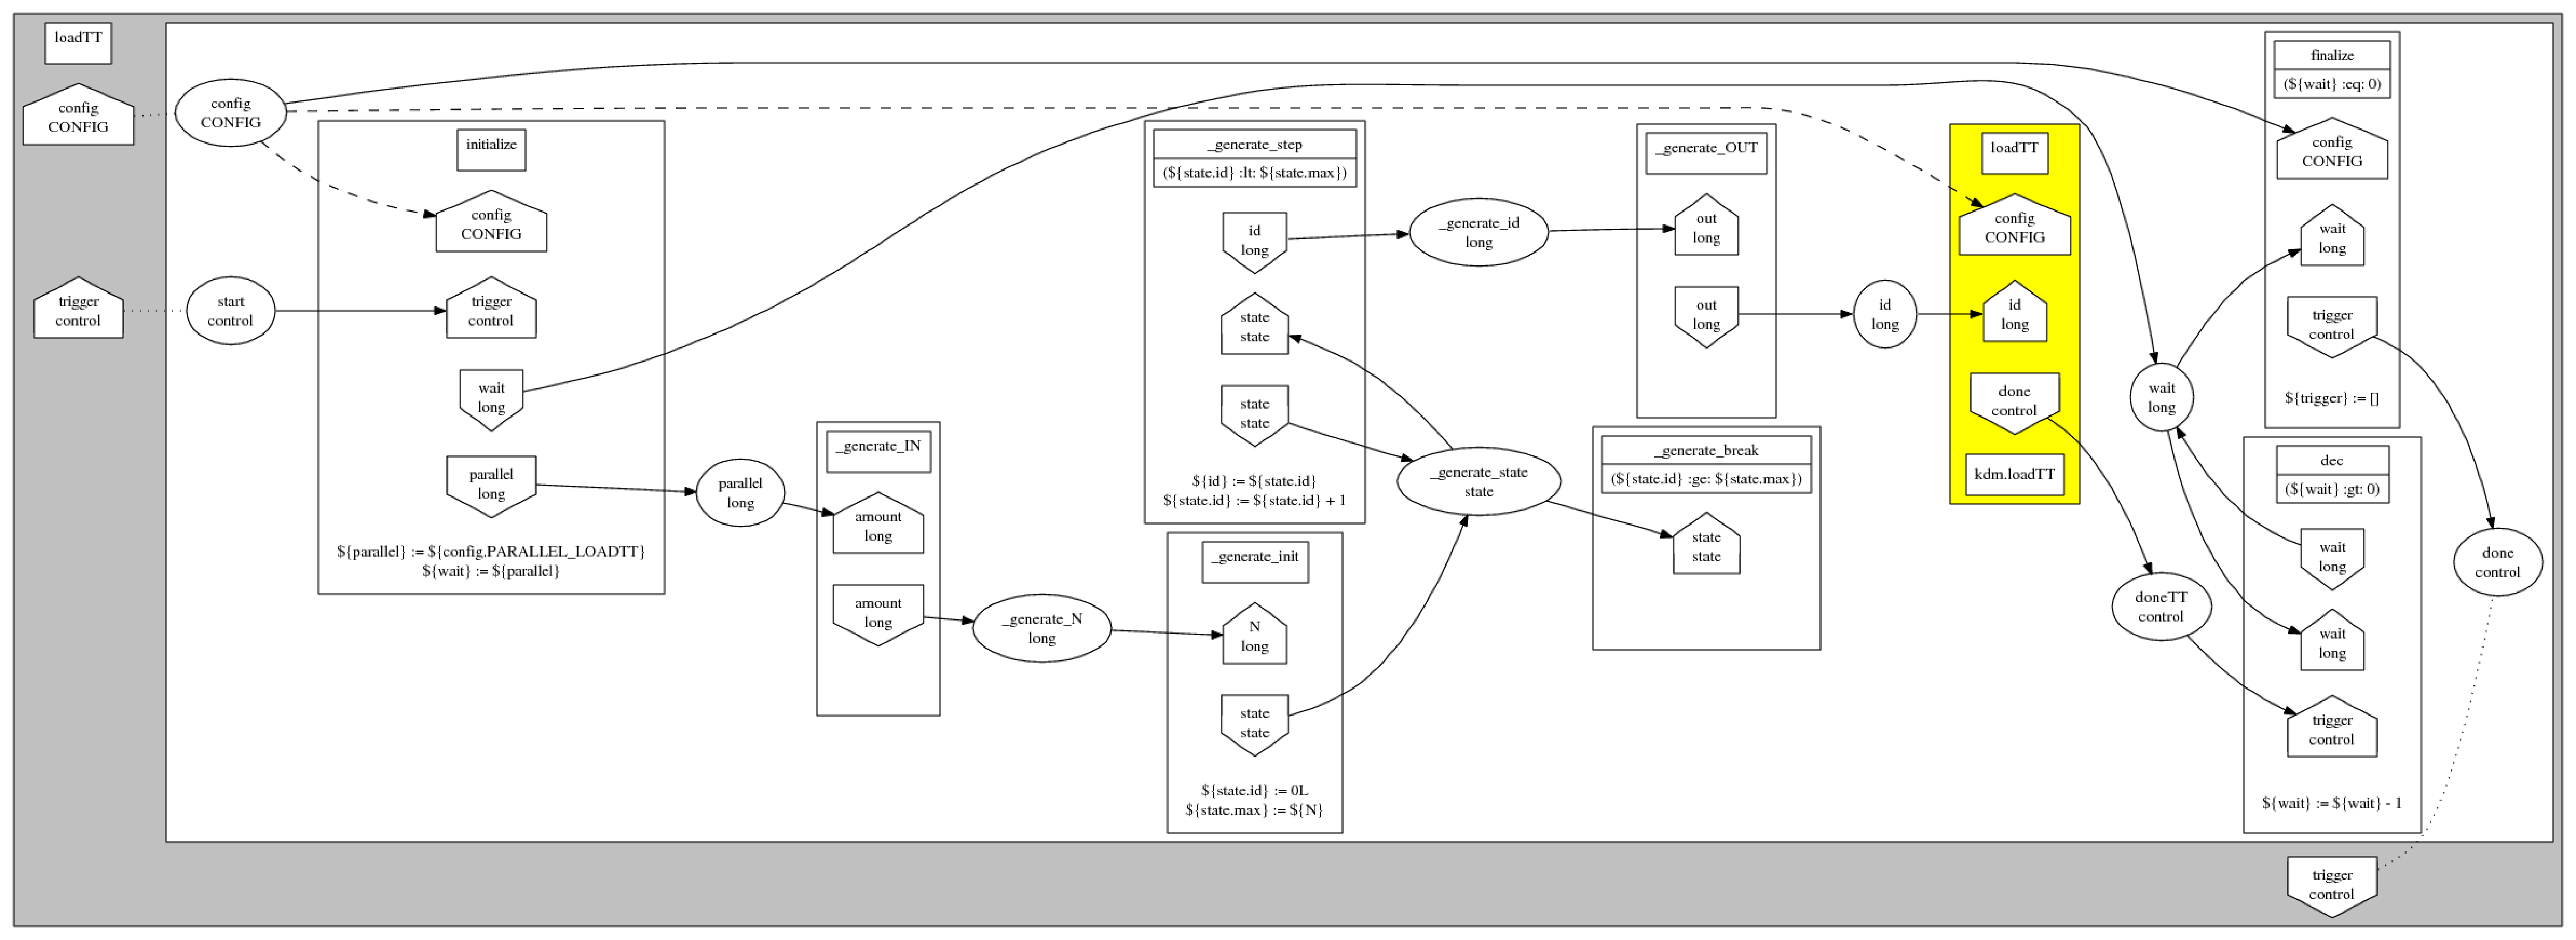
\includegraphics[width=\textwidth]{loadTT_flat.pdf}
\end{center}

Beim Flachklopfen werden \glqq Randtransitionen\grqq\ hinzugef"ugt, im
Beispiel die Transitionen \transition{\_generate\_IN} und
\transition{\_generate\_OUT}, die sichern, dass es im flachgeklopften Netz
eine Schaltreihenfolge gibt, die einer Schaltreihenfolge im nicht
flachgeklopften Netz entspricht.

Eine Transition mu\3 das Attribut \attribute{inline} auf wahr setzen,
um flachgeklopft zu werden.

Der Optimierer von \program{pnetc} kann einige dieser \glqq
Randtransitionen\grqq\ entfernen, im Beispiel ensteht dann das Netz:

\begin{center}
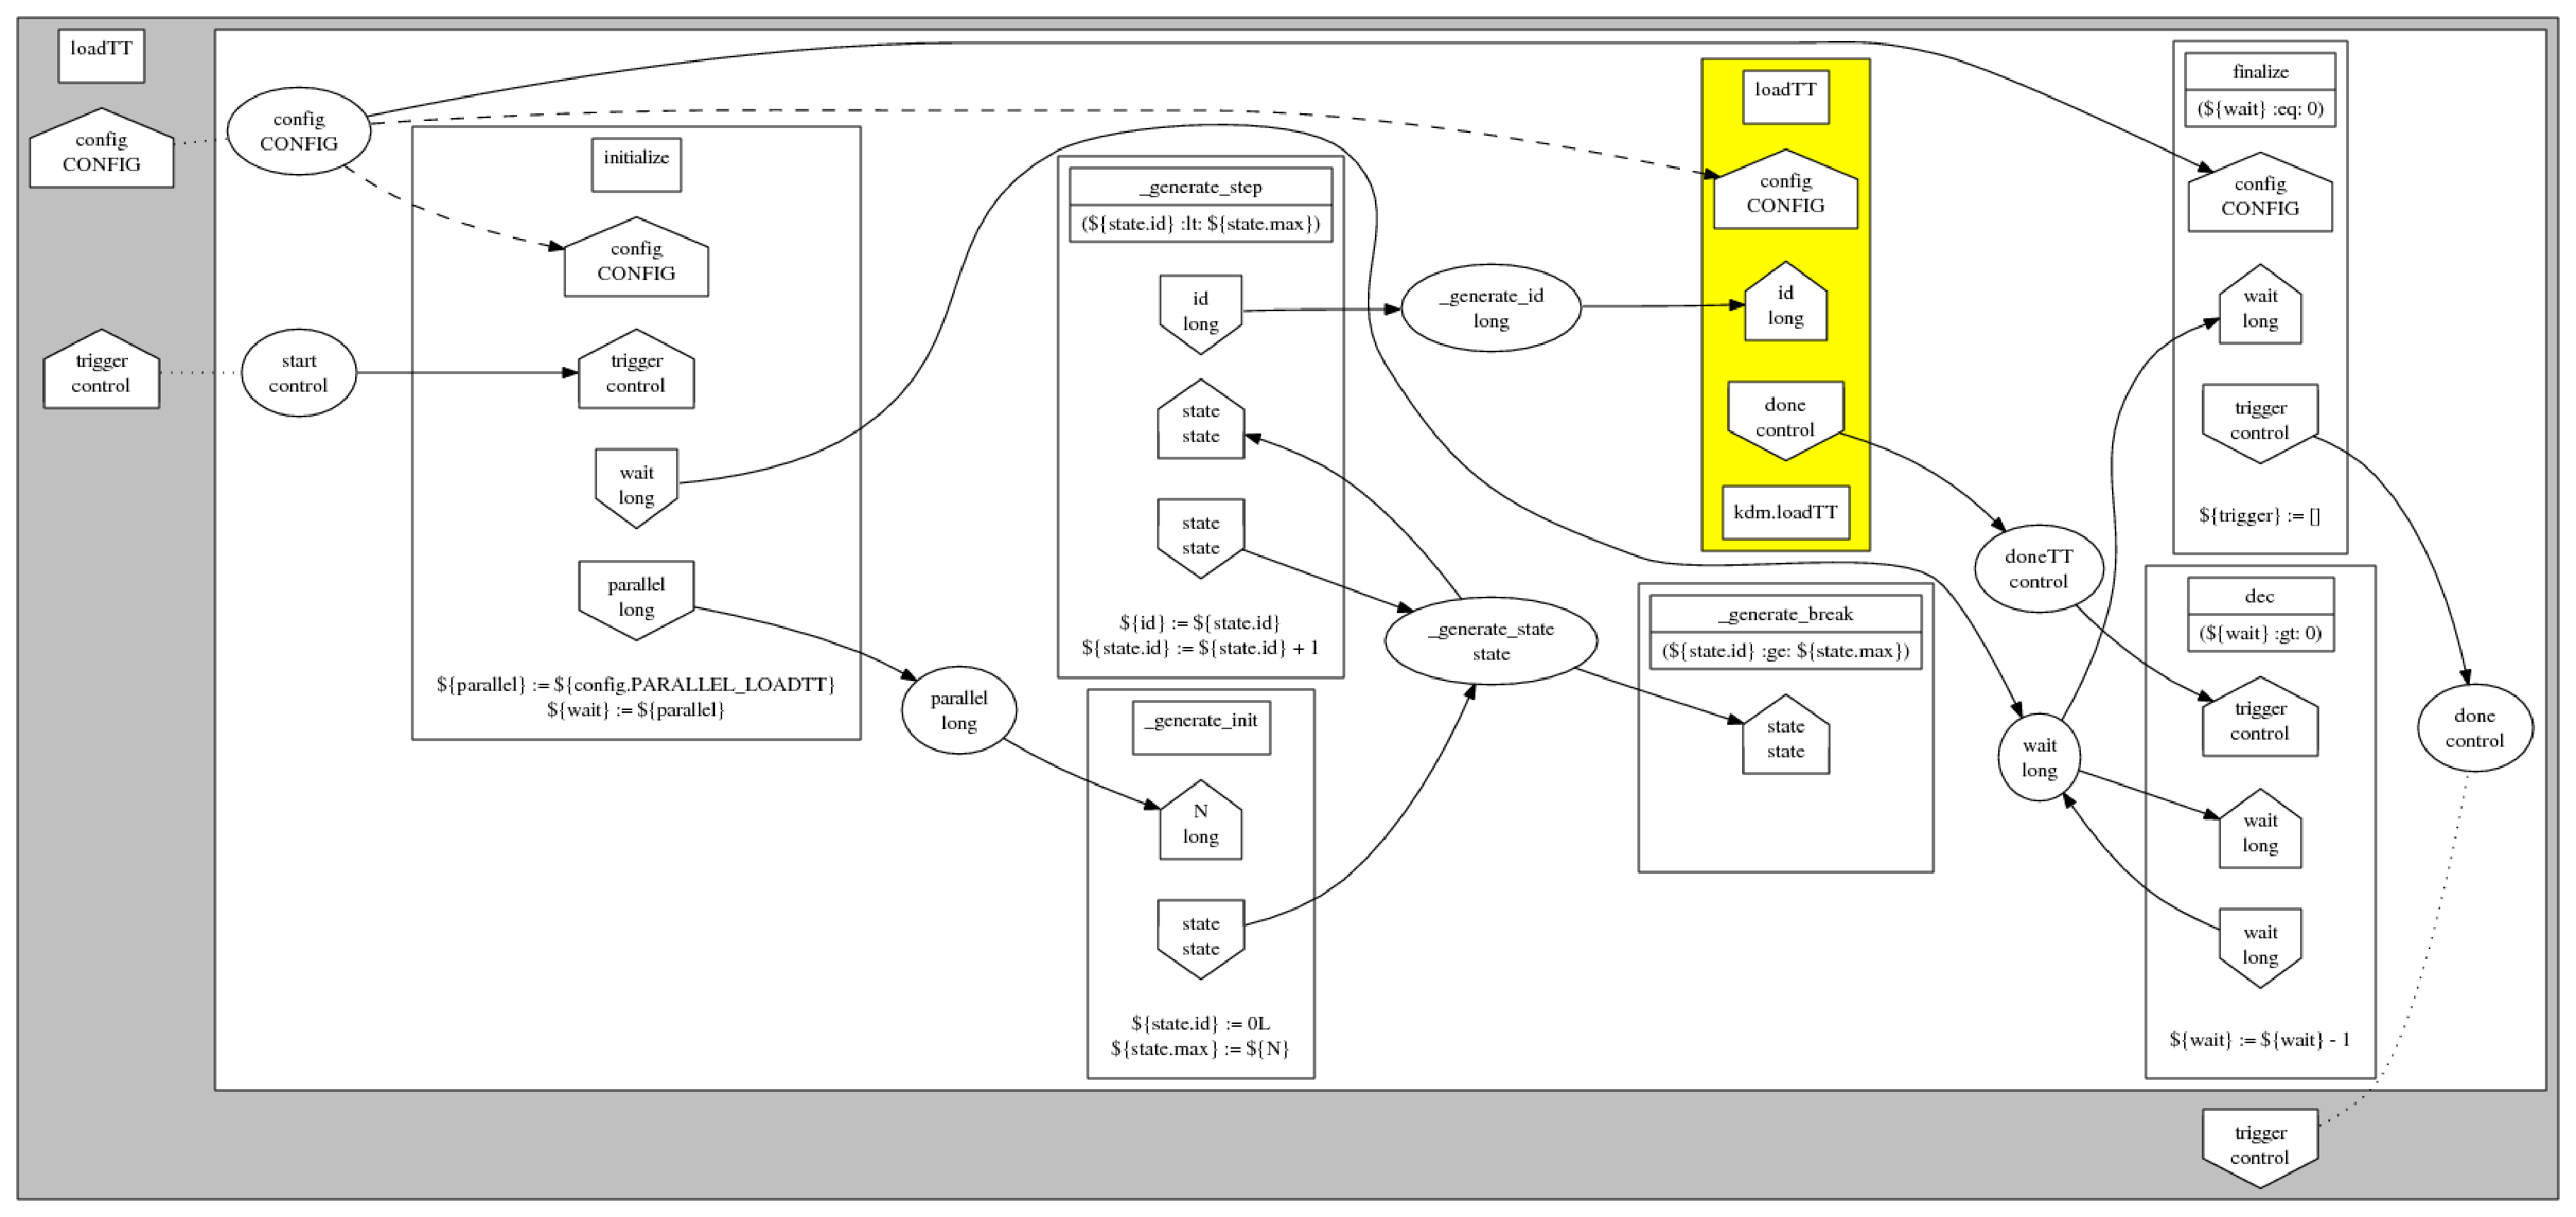
\includegraphics[width=\textwidth]{loadTT_flat_O.pdf}
\end{center}

\section{Das Austauschformat}

Wir haben ein internes (bin"ares) Format und einen Compiler, der XML
lesen und in das interne Format konvertieren kann.

Das XML soll gegen das Schema \file{pnet.xsd} validieren. Dazu
einige Kommentare:

\begin{itemize}

\item Es gibt vier Toplevel-Elemente (\element{defun}, \element{props},
  \element{structs}, \element{template}). Der Compiler erwartet aber
  immer das Element \element{defun} als Toplevel-Element und die anderen
  nur als Toplevel-Element in includierten Dateien. Jeder Workflow ist
  also in \element{defun></defun} eingeschlossen.

\item Es gibt verschiedene M\"oglichkeiten, andere Dateien zu
  includieren. Daf"ur gibt es nicht ein einziges \element{include},
  sondern jeweils angepasste wie \element{include-function},
  \element{include-structs} usw. 

\item An verschiedenen Stellen ist es erlaubt, Properties an die
  Elemente anzuh"angen. Properties sind dabei einfach rekursive
  String->String Abbildungen. Diese Properties k"onnen genutzt werden,
  um Komponenten zu steuern. Im Beispielnetz \file{simple\_kdm.xml}
  steuern wir damit zum Beispiel den Parser und den Pretty Printer.

  Ein Editor kann Properties benutzen, um Layoutinformationen zu
  speichern:
\begin{verbatim}
<place name="a_place" type="a_type">
  <properties name="pnete">
    <properties name="position">
      <property key="x" value="23.42"/>
      <property key="y">47.11</property>
    </properties>
  </properties>
</place>
\end{verbatim}

\item Die Definition eigener Datentypen ist denkbar einfach:
\begin{verbatim}
<struct name="point">
  <field name="x" type="double"/>
  <field name="y" type="double"/>
</struct>
<struct name="line">
  <field name="start" type="point"/>
  <field name="end" type="point"/>
</struct>
\end{verbatim}
  So definierte Typen werden vom Compiler "ubersetzt und von der
  Workflow-Engine komplett verstanden und in der Typpr"ufung verarbeitet.

\item Token k"onnen strukturiert erzeugt werden
\begin{verbatim}
<place name="lines" type="line">
  <token>
    <field name="start"/>
    <field name="end">
      <field name="x"><value>4</value></field>
      <field name="y"><value>4</value></field>
    </field>
  </token>
</place>
\end{verbatim}
  Hier wird der Startpunkt von Default-Konstruktor erzeugt und der
  Endpunkt auf $(4,4)$ gesetzt. Der Kompiler kann bei der Benutzung
  des Default-Konstruktors warnen, ebenso bei unbekannten Felder usw.

\item Wie bereits gesehen werden Pl"atze in \element{place></place}
  eingeschlossen. Sie haben einen Namen, einen Typ und eventuell eine
  Kapazit"at. Auf Pl"atze k"onnen Token gelegt werden.

\item Das Element \element{defun} beschreibt Funktionen. Diese
  Funktionen sind noch keine Transitionen, sondern lediglich die
  Definition von Eingangs- und Ausgangsports, und von
  Ausdruck/externem~Modul/Subnetz.
\begin{verbatim}
<defun name="dup">
  <in name="in" type="long"/>
  <out name="1" type="long"/>
  <out name="2" type="long"/>
  <expression>
    ${1} := ${in};
    ${2} := ${in}
  </expression>
</defun>
\end{verbatim}

\item Im Element \element{transition} wird dann eine Funktion
  verwendet und verbunden. Verbindungen bestehen zwischen Pl"atzen und
  Ports.
\begin{verbatim}
<place name="x" type="long"/>
<place name="y" type="long"/>
<place name="z1" type="long"/>
<place name="z2" type="long"/>
<transition name="dup_x">
  <use name="dup"/>
  <connect-in port="in" place="x"/>
  <connect-out port="1" place="z1"/>
  <connect-out port="2" place="z2"/>
</transition>
<transition name="dup_y">
  <use name="dup"/>
  <connect-in port="in" place="y"/>
  <connect-out port="1" place="z1"/>
  <connect-out port="2" place="z2"/>
</transition>
\end{verbatim}

  Hier wird die Funktion \function{dup} wiederverwendet.

\item Schlie\3lich k"onnen Netze innerhalb von \element{net></net}
  stehen. Die komplette Definition der Funktion, die in der Transition
  \transition{generate} im Beispiel in Abschnitt \ref{sec:hierarchy}
  verwendet wird, sieht so aus:
\begin{verbatim}
<defun>
  <in name="amount" type="long" place="N"/>
  <out name="out" type="long" place="id"/>

  <net>
    <struct name="state">
      <field name="id" type="long"/>
      <field name="max" type="long"/>
    </struct>

    <place name="N" type="long"/>
    <place name="state" type="state"/>
    <place name="id" type="long"/>

    <transition name="init">
      <defun>
        <in name="N" type="long"/>
        <out name="state" type="state"/>
        <expression>
          ${state.id} := 0L; ${state.max} := ${N}
        </expression>
      </defun>
      <connect-in place="N" port="N"/>
      <connect-out port="state" place="state"/>
    </transition>

    <transition name="break">
      <defun>
        <in name="state" type="state"/>
        <expression></expression>
        <condition>${state.id} :ge: ${state.max}</condition>
      </defun>
      <connect-in place="state" port="state"/>
    </transition>

    <transition name="step">
      <defun>
        <in name="state" type="state"/>
        <out name="state" type="state"/>
        <out name="id" type="long"/>
        <expression>
          ${id} := ${state.id}; ${state.id} := ${state.id} + 1
        </expression>
        <condition>${state.id} :lt: ${state.max}</condition>
      </defun>
      <connect-in place="state" port="state"/>
      <connect-out place="state" port="state"/>
      <connect-out place="id" port="id"/>
    </transition>
  </net>
</defun>
\end{verbatim}
\end{itemize}

Das Format ist also insgesamt nicht schwer zu verstehen und alle
weiteren Details finden sich in \file{pnet.xsd}.

Ein Editor soll valides XML erzeugen. Der Compiler \program{pnetc}
f"uhrt mehr Tests durch und kann verwendet werden, um dem Nutzer
R"uckmeldung "uber semantisch inkorrekte bzw.\ zweifelhafte Workflows
zu geben.

\subsection{Templates}

Ein letztes Feature ist die M"oglichkeit, auf XML-Ebene Templates zu
definieren und zu spezialisieren. Ein Template ist dabei prinzipiell
eine Funktion, die aber nicht in \element{defun></defun}, sondern in
\element{template></template} eingeschlossen ist.
\begin{verbatim}
<template name="dup">
  <in name="in" type="T" place="x"/>
  <out name="one" type="T" place="a"/>
  <out name="two" type="T" place="b"/>

  <net>
    <place name="x" type="T"/>
    <place name="a" type="T"/>
    <place name="b" type="T"/>

    <transition name="dup">
      <defun>
        <in name="x" type="T"/>
        <out name="a" type="T"/>
        <out name="b" type="T"/>
        <expression>
          ${a} := ${x};
          ${b} := ${x};
        </expression>
      </defun>
      <connect-in port="x" place="x"/>
      <connect-out port="a" place="a"/>
      <connect-out port="b" place="b"/>
    </transition>
  </net>
</template>
\end{verbatim}

Das Template \function{dup} kann Token beliebiges Typs duplizieren.

Der Compiler kann ein Template zun"achst nicht als Funktion
verwenden. Es mu\3 vorher spezialisiert werden:

\begin{verbatim}
[...]
    <place name="N" type="long"/>
    <place name="produce" type="long"/>
    <place name="consume" type="long"/>

    <include-template href="lib/dup.xml"/>
    <specialize name="dup_long" use="dup">
      <type-map replace="T" with="long"/>
    </specialize>

    <transition name="dup" inline="true">
      <use name="dup_long"/>
      <connect-in port="in" place="N"/>
      <connect-out port="one" place="produce"/>
      <connect-out port="two" place="consume"/>
    </transition>
[...]
\end{verbatim}

Hier wird die Funktion \function{dup\_long} als Spezialisierung des
Templates \function{dup} definiert und verwendet.

Mit Templates k"onnen auch Typen ausgerechnet werden. Das Template
\begin{verbatim}
<template name="tagged_sequence">
  <struct name="PAIR">
    <field name="tag" type="T"/>
    <field name="id" type="long"/>
  </struct>

  <in name="tag" type="T" place="tag"/>
  <in name="amount" type="long" place="N"/>
  <out name="pair" type="PAIR" place="pair"/>

  <net>
    [...]
  </net>
</transition>
\end{verbatim}

erwartet als Eingabe einen Wert $n$ vom Typ \type{long} und ein Tag
$t$ beliebigen Typs \type{T}. Es erzeugt die Liste $(t,0)$, $(t,1)$,
\ldots, $(t,n-1)$. Diese Liste enth"alt Paare des Typ
\type{(T,long)}. Dieser Typ wird innerhalb des Templates definiert und
kann bei Spezialisierung ausgelesen werden.
\begin{verbatim}
[...]
    <place name="amount" type="long"/>
    <place name="volume" type="VOLUME"/>
    <place name="pair" type="pair_long_VOLUME"/>

    <include-template href="tagged_sequence.xml"/>
    <specialize name="tag_seq" use="tagged_sequence">
      <type-map replace="T" with="VOLUME"/>
      <type-map replace="PAIR" with="pair_long_VOLUME"/>
      <type-get name="pair_long_VOLUME"/>
    </specialize>

    <transition name="tag_seq" inline="true">
      <use name="tag_seq"/>
      <connect-in port="tag" place="volume"/>
      <connect-in port="amount" place="amount"/>
      <connect-out port="pair" place="pair"/>
    </transition>
[...]
\end{verbatim}

Hier wird das Template \function{tagged\_sequence} benutzt und der vom
Template berechnete Typ \type{pair\_long\_VOLUME} wird ausgelesen und
verwendet.

Der Template-Mechanismus funktioniert im Prinzip genauso wie in
C++. Im Beispiel \file{simple\_kdm.xml} wird davon Gebrauch gemacht.

\section{Vorhandene Programme}

F"ur komplette Parameterlisten jeweils \texttt{----help}.

\subsection{\program{pnetc}}\label{sec:pnetc}

Der bereits erw"ahnte Compiler. Liest XML Files und produziert Dateien
im internen Format. Die Plattform arbeitet nur mit Daten im internen
Format. Das hei\3t, s"amtliche Fehler und Warnungen des Compilers
sollte der Editor an die Nutzerinnen weitergeben oder selbst
verarbeiten. Im Moment handelt es sich bei den Fehlermeldungen eingach
um den Text von Ausnahmen. Hier kann bei Bedarf auch eine andere
Schnittstelle implementiert werden.

\subsection{\program{pnet2dot}}\label{sec:pnet2dot}

Liest Daten im internen Format und produziert Ausgabe in
DOT. (\url{www.graphviz.org}) Macht Gebrauch von der
Clustering-F"ahigkeit des Programms \program{dot}. Die erzeugten
Layouts sind nicht soo schlecht.

Zusammen mit \program{pnetc} eine komplette
Entwicklungsumgebung. Interessant, die M\"oglichkeit, Transitionen nur
bedingt anzuzeigen. Die Kommandzeile
\begin{verbatim}
pnetc loadTT.xml -Iapplication/ --no-inline yes |\
pnet2dot --not-starts-with=generate             |\
dot -Tps -Grankdir=LR
\end{verbatim}
erzeugt das Bild
\begin{center}
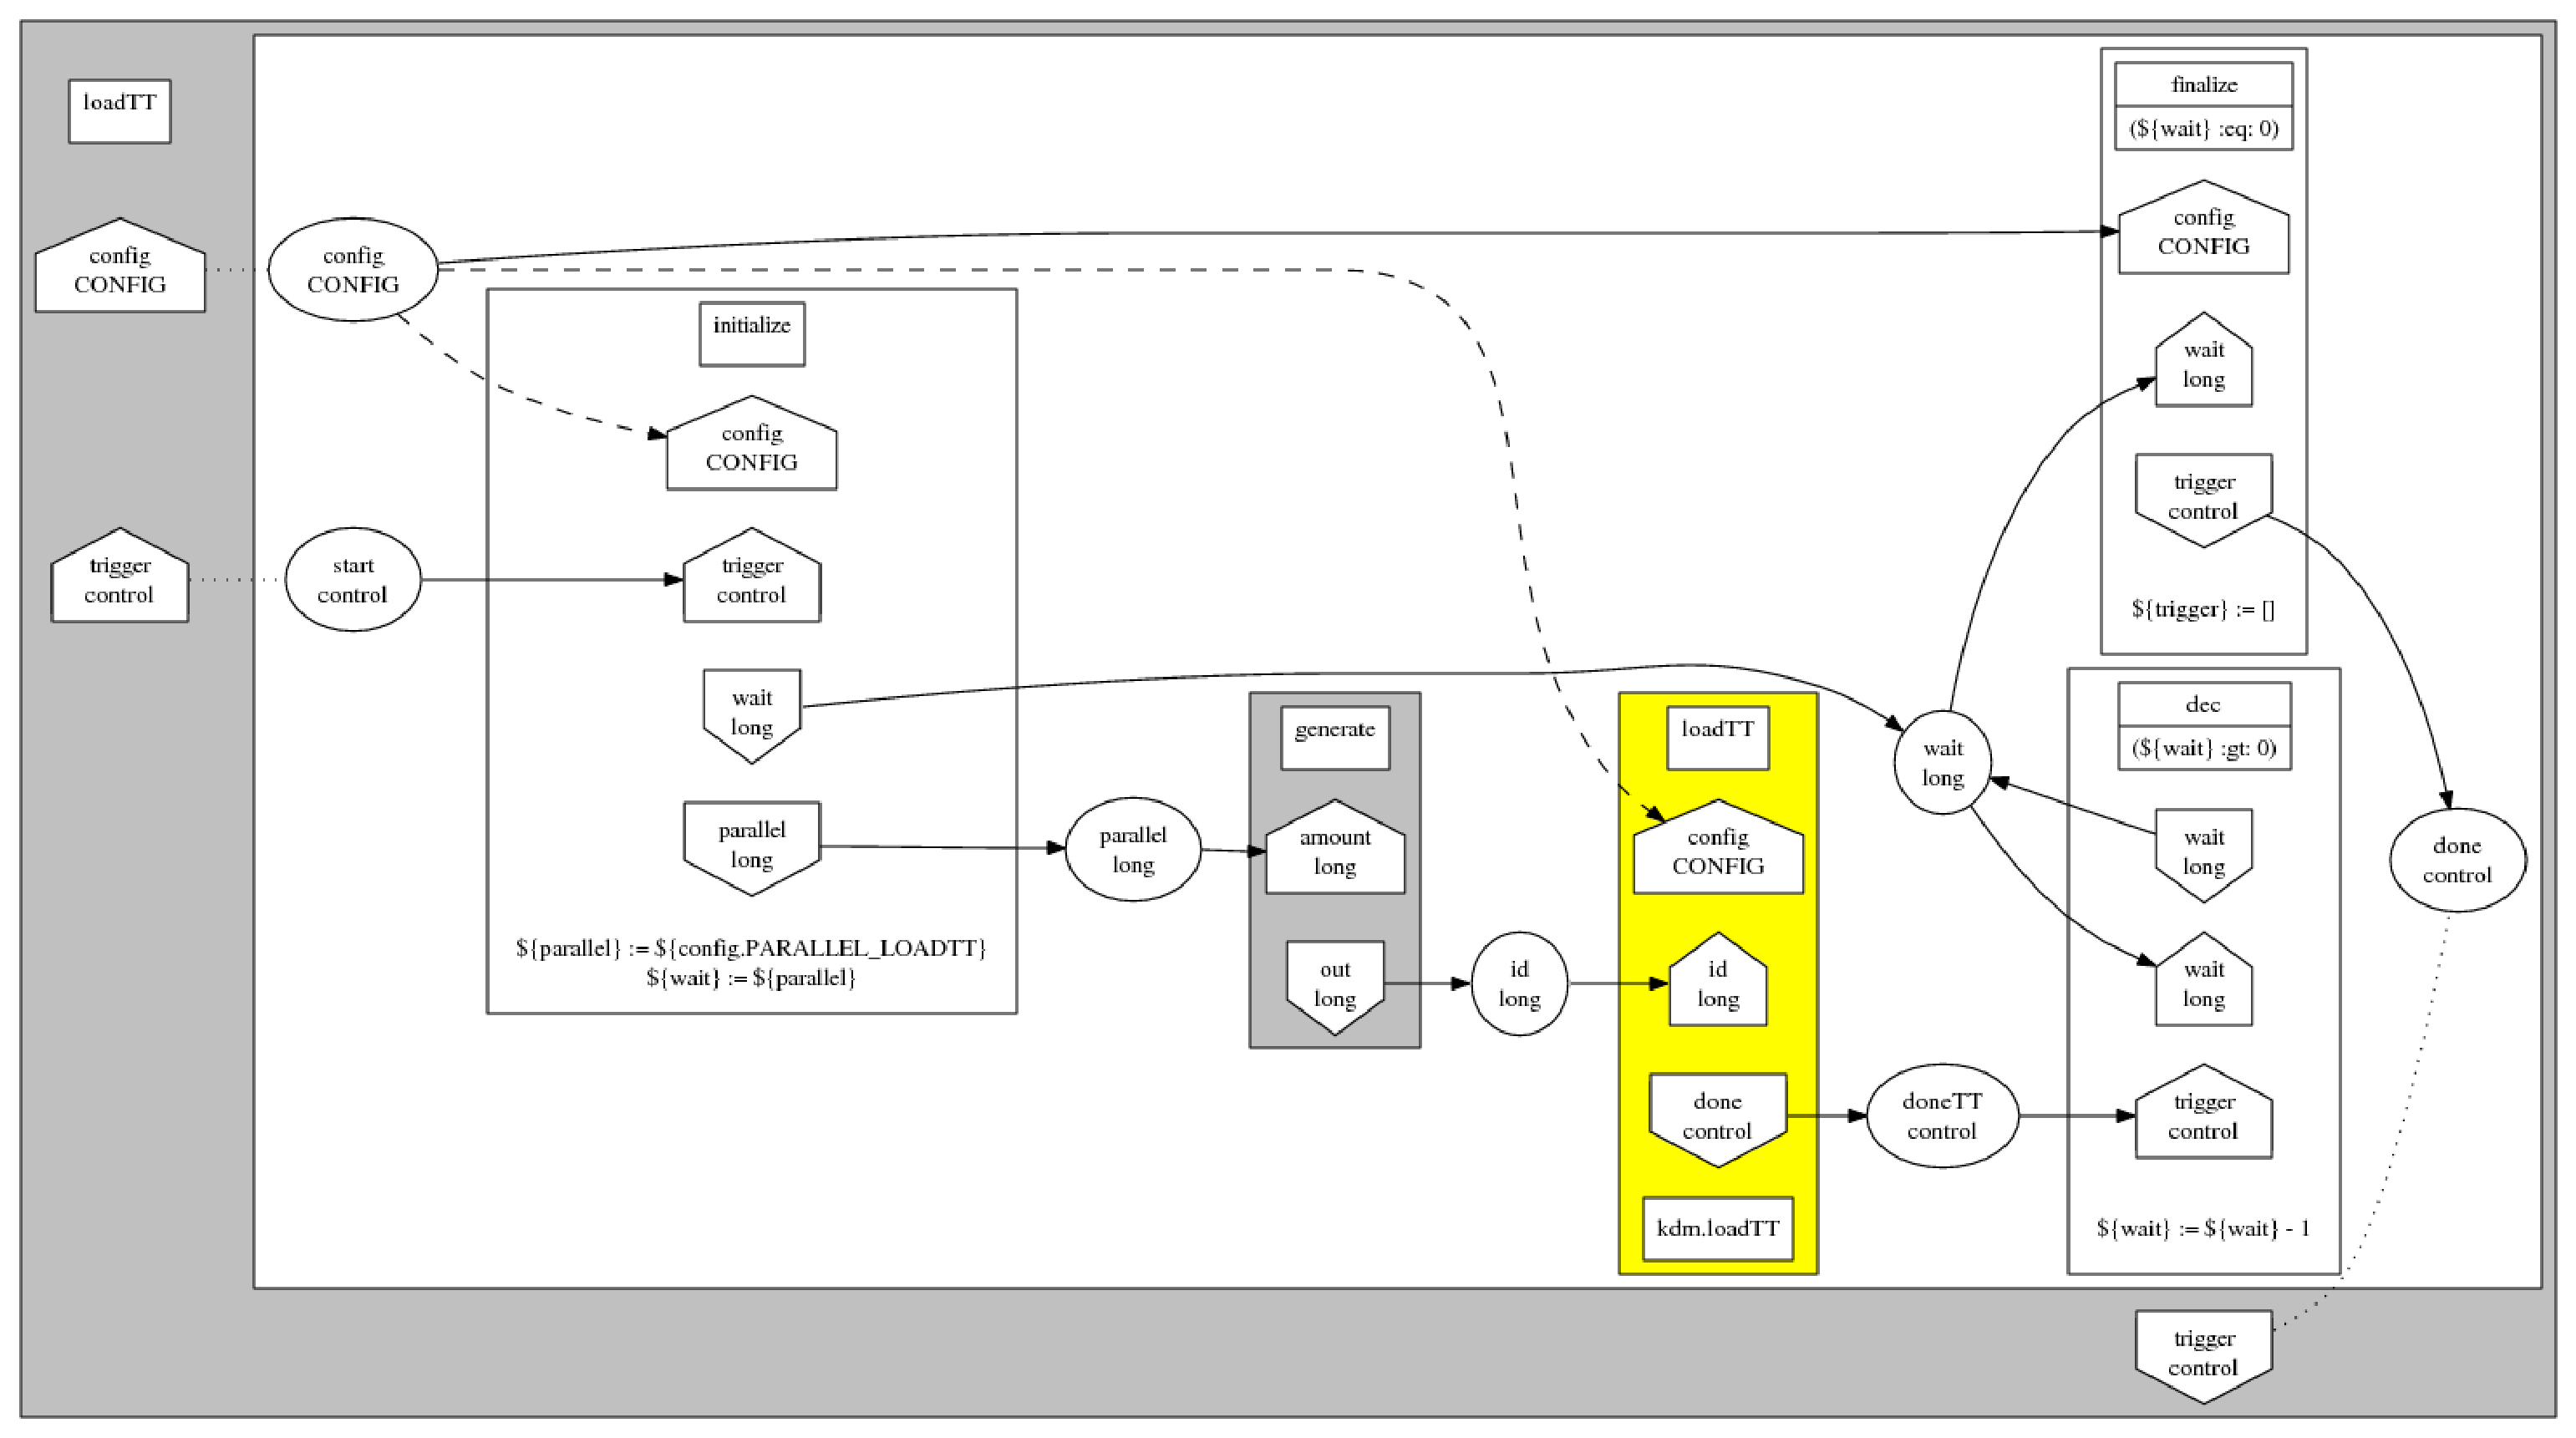
\includegraphics[width=\textwidth]{loadTT_concept.pdf}
\end{center}
Das ist wieder das Netz aus Abschnitt \ref{sec:hierarchy}, aber der
Subworkflow \transition{generate} wird nicht detailliert dargestellt.

So stellen wir uns das Ein- und Ausblenden von Subnetzen vor.

\section{Der Editor}

\subsection{Stand der Dinge: Plattformexperte}\label{sec:use:today}

Im Moment besteht die Entwicklungsumgebung aus einem Texteditor der
Wahl und den beiden Programmen \program{pnetc} und \program{pnet2dot}.

Es wird im Texteditor direkt eine XML-Datei bearbeitet. Diese
XML-Datei dient als Eingabe f"ur den Compiler. Dessen Fehlermeldungen
und Warnungen werden h"andisch begutachtet und eventuell wird die
XML-Datei angepasst.

Ist der Compiler zufrieden, wird das Programm \program{pnet2dot}
benutzt, um ein grafisches Feedback des Workflows zu generieren. Falls
hier nicht alles so ist, wie sich bei der Eingabe der XML-Datei
vorgestellt wurde, wird erneut die XML-Datei modifiziert.

Entspricht die XML-Datei den Vorstellungen, wird der Workflow
getestet:
\begin{itemize}
\item mit Hilfe des Programms \program{we-exec}, dass einen Workflow
  ausf"uhren kann, ohne die gesamte Umgebung der Plattform zu
  ben"otigen

\item mit Hilfe eines Simulators, der die gesamte Plattform auf
  einzelnen Rechenknoten simulieren kann. Der Simulator ist dabei im
  Prinzip nicht von der eigentlichen Plattform zu unterscheiden und
  verwendet exakt die selben Bausteine. Lediglich der virtuelle
  Speicher wird simuliert.

\item mit Hilfe der gesamten Plattform inklusive echtem virtuellen
  Speicher.
\end{itemize}

Werden Workflows mit externen Modulen editiert, dann sind
Plattformexperten in der Lage auch diese Module zu modifizieren und
gegebenfalls Testmodule zu erstellen.

Der Stand der Dinge ist nicht zufriedenstellend:
\begin{itemize}
\item Der Zyklus von XML-Datei zum grafischen Feedback ist zu lang.
\item Anwenderwissen kann nur "uber den Umweg des Plattformexperten in
  Workflows eingebracht werden.
\item Kleine "Anderungen an Workflows erfordern zu viel Zeit.
\item Nur Experten finden sich zurecht.
\end{itemize}

Im Moment gibt es genau zwei Personen, die hier volles Verst"andnis
haben. Eine dritte Person benutzt diese Umgebung und hilft bei der
Identifizierung der Schwachstellen. Alle drei Personen wollen gern
einen Editor wie im folgenden Abschnitt beschrieben.

\subsection{Petri-Netz Entwickler: Koordinierungsexperte, Plattformanwender}

Nutzerin oder Nutzer ist Spezialistin oder Spezialist f"ur den
Koordinationslevel. Sie oder er versteht die Feinheiten, die bei der
Programmierung von Petri-Netzen zu beachten sind vollst"andig. Alle
Details der Plattform werden verstanden und beherrscht. Die Plattform
selber steht zum Testen separat vom Editor zur Verf"ugung, zusammen
mit Werkzeugen wie Compiler oder Simulator. Externe Module liegen vor
und werden nicht erstellt oder modifiziert.

Der Editor wird benutzt, um grafisch erweiterte Petri-Netze zu
editieren. Editorobjekte sind Pl"atze und Transitionen. Alle
Erweiterungen sind komplett im Editor ansprechbar, also zum Beispiel
Ports und Typen. Der Editor erlaubt die Definition eigener Datentypen
und von Token solcher Typen. Der Editor hat Basisfunktionalit"at zum
Umgang mit hierarchischen Netzen, also zum Beispiel Ein- und
Ausblenden von Subnetzen. Der Editor organisiert Workflows in Ordnern
und Bibliotheken. Der Editor kann XML-Dateien schreiben und lesen. Er
speichert Layoutinformationen als properties der Elemente. Er kann
XML-Dateien ohne Layoutinformationen lesen und erzeugt automatisch ein
Layout.

Die Ausgabe des Editors ist eine XML-Datei, die dann wie in
\ref{sec:use:today} benutzt wird.

Der Editor ben"otigt keinerlei Anbindung an die Plattform oder Teile
der Plattform. Fehlermeldungen des Compilers werden h"andisch
begutachtet. Tests werden h"andisch durchgef"uhrt. Eine einfache
Einbindung des Compilers ist jedoch w"unschenswert.

Im Unterschied zu \ref{sec:use:today} verk"urzt sich die
Entwicklungszeit erheblich, da durch das Verbleiben auf der grafischen
Ebene nicht mehr der gedankliche Umstieg auf das XML-Format erfolgen
mu\3.

\subsection{Editor f"ur Dom"ananwender: Dom\"anexperte, Koordinierungsanwender}

Nutzerin oder Nutzer ist Spezialistin oder Spezialist f"ur die Dom"an
und hat ein Verst"andnis der Koordinierungsschicht. Die Plattform ist
in Grundz"ugen bekannt. Petri-Netze sind nicht bekannt, insbesondere
keine Details. Die Plattform und Bausteine sind verf"ugbar. Externe
Module liegen vor.

Der Editor wird benutzt, um grafisch Dom"anapplikationen zu
erstellen. Editierobjekte sind Repr"asenationen von
Dom"anobjekten. Der Formalismus Petri-Netz ist nicht sichtbar,
bzw. ist sichtbar wo sinnvoll und dann nicht zwingend als solcher
gekennzeichnet. Konzepte wie Typen und Ports werden vom Editor
transparent behandelt und beachtet. Der Compiler ist voll integriert,
Fehler und Warnung werden auf die Dom"an "ubertragen und grafisch
dargestellt. Der Editor baut auf Workflows und Bibliotheken auf, die
Plattformexperten zur Verf"ugung stellen. Der Editor gestattet die
Definition neuer Typen. Der Editor organisiert Workflows in Ordnern
und Bibliotheken. Der Editor verwendet eventuell ein anderes
Speicherformat als die Plattform XML-Dateien. Er kann aber Plattform
XML-Dateien schreiben und lesen.

Der Editor hat eine einfache Anbindung an die Plattform und gestattet
direkt das Ausf"uhren eines Workflows in der Plattform oder im
Simulator. Er stellt Funktionalit"at zur Verf"ugung, um Parameter im
Workflow einzustellen. Die Beobachtung laufender Workflows erfolgt
durch externe Programme. Eine einfache Einbindung solcher Programme
ist jedoch w"unschenswert.

\subsection{Exploratives Entwickeln: Dom"ananwender}

Nutzerin oder Nutzer ist Dom"ananwender. Die Plattform ist im
wesentlichen unbekannt. Petri-Netze sind unbekannt. Die Plattform ist
verf"ugbar. Externe Module liegen vor.

Der Editor wird benutzt, um grafisch mit Dom"anobjekten zu
operieren. Editierobjekte sind Repr"asenationen von
Dom"anobjekten. Die gesamte Plattform ist vollst"andig integriert. Der
Editor erlaubt nur korrekte Workflows, das hei\3t, Fehlermeldungen und
Warnungen des Compilers werden vom Editor bearbeitet und dringen nicht
bis zum Nutzer oder zur Nutzerin vor. Der Editor baut of Workflows und
Bibliotheken auf, die Dom"anexperten zur Verf"ugung stellen. Ziel ist
nicht die Erzeugung eines Workflows, sondern der Umgang mit Objekten
der Dom"an. Dabei entsteht \glqq nebenbei\grqq\ auch ein Workflow, der
auch gespeichert werden kann, zum Beispiel zur Weiterverwendung mit
anderen Parametern oder zur Optimierung durch Plattformanwenderinnen
oder -experten.

Mindestens: Die Beobachtung laufender Workflows kann durch externe
Programme erfolgen. Die Einbindung solcher Programme ist sehr
sinnvoll. Eigene Funktionalit"at zur Beobachtung laufender Workflows
ist w"unschenswert.

Gew"unscht: Die Beobachtung laufender Workflows erfolgt durch interne
Komponenten des Editors. Die Nachrichten und Ereignisse werden dabei
in die Dom"an "ubertragen. Es ist keine Kenntnis der Plattform n"otig.

\section{Der Monitor}

Neben dem Editor ist der Monitor eine wichtige Komponente. Im Moment
haben wir ein sehr einfaches Programm, das grafisch "uber
Basisaktivit"aten informiert. Petri-Netze bieten prinzipiell die
M"oglichkeit, den Zustand eines laufenden Workflows direkt
darzustellen: Die Token repr"asentieren Daten und deren Position im
Netz beschreibt den Bearbeitungsstand. Das hei\3t, dass ein Editor und
ein Monitor die selbe Oberfl"ache haben k"onnen und sollten.

Im Anwendungsszenario \glqq Exploratives Entwickeln\grqq\ ist eine
komplette Integration eines Monitors in den Editor sehr sinnvoll.

Der Monitor soll einerseits den Fortschritt eines Workflows darstellen
und andererseits die Beobachtung der Maschine erm"oglichen.

Es gibt hier viele offene Fragen: Wie mit Hierarchien umgehen? Wie mit
sehr vielen Ereignissen? Was genau interessiert die Anwenderinnen und
Anwender? Wie kann das dem System mitgeteilt werden?

\renewcommand{\bibname}{Literatur}
\begin{thebibliography}{\quad}

\bibitem{gelernter}D.~Gelernter, N.~Carriero. \emph{Integration or
    Separation.} Communications of the ACM 35(2):97--107, 1992.

\end{thebibliography}

\end{document}